% questions.tex —— 1977 年·广西百色卷（理科） · 题目内容片段（无答案）
% 由 tools/generate_projects.py 依来源总账自 1977/1977_数学真题_广西百色理_试题.md 生成，勿手改（改源 MD 后重跑）


\gkpart{广西百色试点（理科）}

\begin{gktip}
\textbf{来源说明}：本题面依据固定源 PDF《1977广西百色理》第 1—6 页（书页 141—146）逐题转录。固定源是题面与解答连排的书籍材料：每题题面后紧跟「解」「证明」「答」，并非空白试卷；本文只转录题面，配套答案与解析由本库对照源解答独立复算推导，\textbf{非官方标准答案}。原卷按大题「一、」至「六、」编号，第一大题、第二大题下各有 4 个小题，第三大题下有 2 个小题；本库将大题重排为连续题号 1—6，大题内小题统一为（1）（2）…小问格式，未增删题干。原卷未标分值。卷末第六题后印有「选作题：」栏（2 题），本库按参考题处理，不计入正式题量。第 5 题求证第一式把角 $C$ 排成小写「cosc」，系排印之误，详见该题源注。
\end{gktip}

\begin{question}
\gkti{1}

（1） 求函数 $y=\dfrac{2\sqrt{5-x}}{\sqrt{x-3}}$ 的定义域。

\Needspace{5\baselineskip}
（2） 计算：

\nopagebreak[4]
\[
\left(-\frac12\right)^{-3}+32^{\frac25}+5^0-3^{-2}
\]

（3） 求 $\sin^2 60^\circ+\operatorname{ctg}45^\circ+\dfrac34\operatorname{tg}^2 30^\circ-\cos 60^\circ$ 的值。

（4） $\log_2\sqrt8=x$，求 $x$。

\end{question}
\begin{question}
\gkti{2}已知直线过 $(3,1)$ 和 $(-6,4)$ 两点。

（1） 求出这直线方程。

（2） 求它的斜率和 $y$ 轴上的截距。

（3） 这函数是上升或下降。

（4） 求过 $(0,-5)$ 和这直线平行的直线方程。

\Needspace{0.4\textheight}
\end{question}
\begin{question}
\gkti{3}已知圆 $O$ 中两弦 $AB$、$CD$ 相交于 $E$。

（1） 证明 $AE\cdot BE=CE\cdot DE$。

（2） 当 $CD$ 为直径（$2R$），$AB\perp CD$ 时，证明 $BE^2=CE(2R-CE)$。

\begin{gktip}
原源 PDF 第 3 页在本题旁附有圆内两弦相交示意图；LaTeX 版按源图重绘。
\end{gktip}
\nopagebreak[4]
\begin{center}% 1977 年广西百色卷（理科）第三题：圆 O 内两弦 AB、CD 相交于 E，
% 虚线 AC、BD 为证 △AEC∽△DEB 所连（按源卷第 3 页布局）
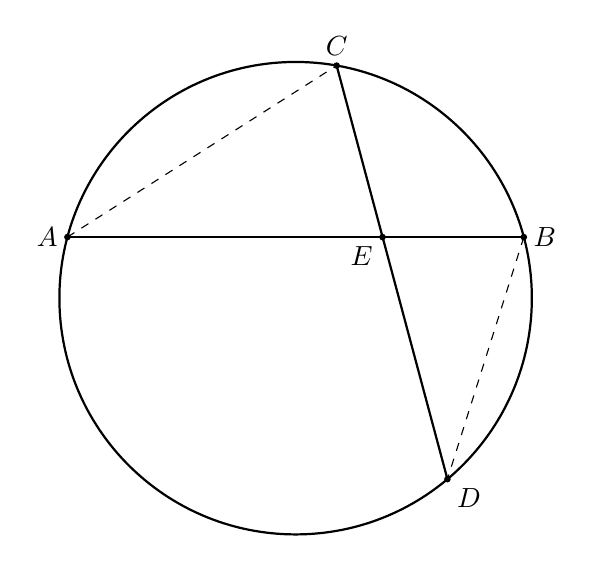
\begin{tikzpicture}[scale=1.0]
  % 圆半径 3cm；A 在 165°、B 在 15°、C 在 80°、D 在 310°
  \draw[thick] (0,0) circle (3);
  \coordinate (A) at (-2.898,0.776);
  \coordinate (B) at (2.898,0.776);
  \coordinate (C) at (0.521,2.954);
  \coordinate (D) at (1.928,-2.298);
  \coordinate (E) at (1.104,0.776); % AB 与 CD 的交点
  \draw[thick] (A)--(B);
  \draw[thick] (C)--(D);
  \draw[dashed] (A)--(C);
  \draw[dashed] (B)--(D);
  \fill (A) circle (1.2pt) node[left] {$A$};
  \fill (B) circle (1.2pt) node[right] {$B$};
  \fill (C) circle (1.2pt) node[above] {$C$};
  \fill (D) circle (1.2pt) node[below right] {$D$};
  \fill (E) circle (1.2pt) node[below left] {$E$};
\end{tikzpicture}
\end{center}
\nopagebreak[4]
\end{question}
\begin{question}
\gkti{4}一船往返于 $48$ 公里的两地，共航行 $10$ 小时，已知水流速度是 $2$ 公里/小时，求这轮船在静水中航行的速度。

\Needspace{0.4\textheight}
\end{question}
\begin{question}
\gkti{5}已知 $A$、$B$、$C$ 是 $\triangle ABC$ 的三个内角，求证

\nopagebreak[4]
\[
\begin{aligned}
&a=b\cos c+c\cos B,\\
&b=c\cos A+a\cos C,\\
&c=a\cos B+b\cos A.
\end{aligned}
\]

\begin{gktip}
\textbf{源注}：源卷把第一式余弦的角排印为小写「c」（印作「a = bcosc + ccosB」），系排印之误，此处保留转录，应读作 $\cos C$。求证的三条式子跨源卷第 4—5 页连排。
原源 PDF 第 4 页在本题旁附有三角形与底边上的高示意图；LaTeX 版按源图重绘。
\end{gktip}
\nopagebreak[4]
\begin{center}% 1977 年广西百色卷（理科）第五题：三角形 ABC 的三边 a、b、c，
% AD 为 BC 边上的高（虚线）（按源卷第 4 页布局）
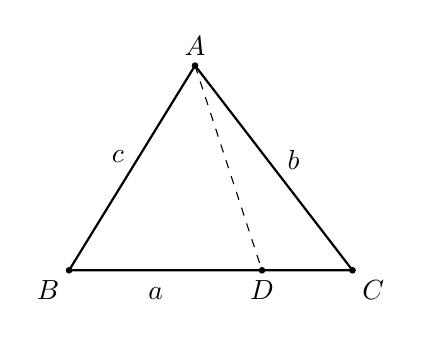
\begin{tikzpicture}[scale=1.0]
  \coordinate (A) at (1.6,2.6);
  \coordinate (B) at (0,0);
  \coordinate (C) at (3.6,0);
  \coordinate (D) at (2.45,0); % 高的垂足
  \draw[thick] (A)--(B)--(C)--cycle;
  \draw[dashed] (A)--(D);
  \fill (A) circle (1.2pt) node[above] {$A$};
  \fill (B) circle (1.2pt) node[below left] {$B$};
  \fill (C) circle (1.2pt) node[below right] {$C$};
  \fill (D) circle (1.2pt) node[below] {$D$};
  \node at (0.62,1.45) {$c$};
  \node at (2.85,1.40) {$b$};
  \node at (1.10,-0.30) {$a$};
\end{tikzpicture}
\end{center}
\nopagebreak[4]
\Needspace{0.4\textheight}
\end{question}
\begin{question}
\gkti{6}当 $a$、$b$、$c$ 为实数时，求证方程 $x^2-(a+b)x+(ab-c^2)=0$ 有两个实数根，并求出两个根相等的条件。

\begin{gktip}
\textbf{参考题说明}：源卷第六题后印有「选作题：」栏，其下两题以「1、」「2、」编号。本库按参考题 1、2 处理，不计入正式题量。
\end{gktip}

\Needspace{5\baselineskip}
\textbf{参考题 1．} 已知：

\nopagebreak[4]
\[
2\lg(x-2y)=\lg x+\lg y,
\]

求：$x:y$。

\textbf{参考题 2．} 求内接于半径为 $10$ 厘米，圆心角为 $120^\circ$ 的弓形的正方形的边长。

\begin{gktip}
原源 PDF 第 6 页在本题旁附有弓形内接正方形示意图；LaTeX 版按源图重绘。
\end{gktip}
\nopagebreak[4]
\begin{center}% 1977 年广西百色卷（理科）参考题 2（源卷「选作题」第 2 题）：半径 10cm、
% 圆心角 120° 的弓形内接正方形 CDEF，半径 OP⊥FE 交 FE 于 N、AB 于 M（按源卷第 6 页布局）
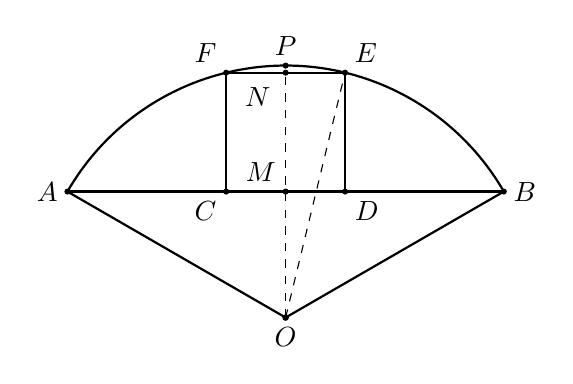
\begin{tikzpicture}[scale=1.0]
  % O 为圆心，R=3.2cm；A、B 为弦端点，C、D 在弦上，F、E 在弧上，P 为弧中点
  \coordinate (O) at (0,0);
  \coordinate (A) at (-2.771,1.6);
  \coordinate (B) at (2.771,1.6);
  \coordinate (M) at (0,1.6);
  \coordinate (C) at (-0.755,1.6);
  \coordinate (D) at (0.755,1.6);
  \coordinate (N) at (0,3.110);
  \coordinate (F) at (-0.755,3.110);
  \coordinate (E) at (0.755,3.110);
  \coordinate (P) at (0,3.2);
  \draw[thick] (O)--(A);
  \draw[thick] (O)--(B);
  \draw[thick] (A)--(B);
  \draw[thick] (A) arc (150:30:3.2);
  \draw[thick] (C)--(F)--(E)--(D);
  \draw[dashed] (O)--(P);
  \draw[dashed] (O)--(E);
  \fill (O) circle (1.2pt) node[below] {$O$};
  \fill (A) circle (1.1pt) node[left] {$A$};
  \fill (B) circle (1.1pt) node[right] {$B$};
  \fill (P) circle (1.1pt) node[above] {$P$};
  \fill (F) circle (1.1pt) node[above left] {$F$};
  \fill (E) circle (1.1pt) node[above right] {$E$};
  \fill (C) circle (1.1pt) node[below left] {$C$};
  \fill (D) circle (1.1pt) node[below right] {$D$};
  \fill (M) circle (1.1pt) node[above left] {$M$};
  \fill (N) circle (1.1pt) node[below left=2pt] {$N$};
\end{tikzpicture}
\end{center}
\nopagebreak[4]

\end{question}